\documentclass{article}
\usepackage{graphicx}

\title{Data visualizations and metrics}
\date{2024-10-17}
\author{Andrew Bartnof, for RMI}
\begin{document}
  \maketitle

\section{Introduction}

In the near future, we'll chat about the tools, metrics, and visual metaphors that will allow us to explore the data underlying Jeremy's Energy Communities initiative.
Jeremy's job is to get you fired up about how we can help people-- my job, thankfully, is just to get you thinking about the visual tools that you'd love to explore.

I have written this article in a \LaTeX\ pdf for a few silly reasons: 
\begin{itemize}
\item I have been working with Google's interactive dashboard system, but it's not ready for primetime yet. In contrast, I can always present something to you in R/GGPlot.
\item I don't think I have the ability to make a new Microsoft Office document anymore using our Teams setup.
\end{itemize}

\section{Data, and useful visual metaphors}

The two datasets that we'll focus on right now are foundational for this project: Clean Repowering, and the Clean Investment Monitor.
\begin{figure}
  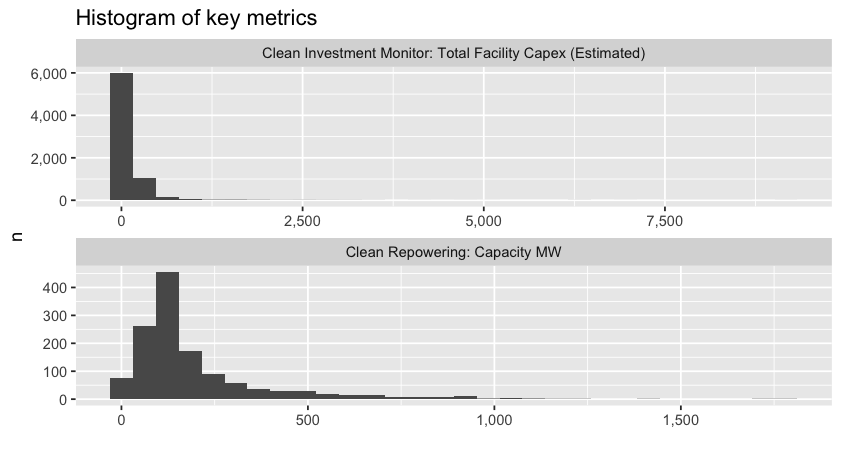
\includegraphics[width=\linewidth]{images/histograms.png}
  \caption{The overall distribution of key metrics in our two datasets}
\end{figure}

\begin{figure}
  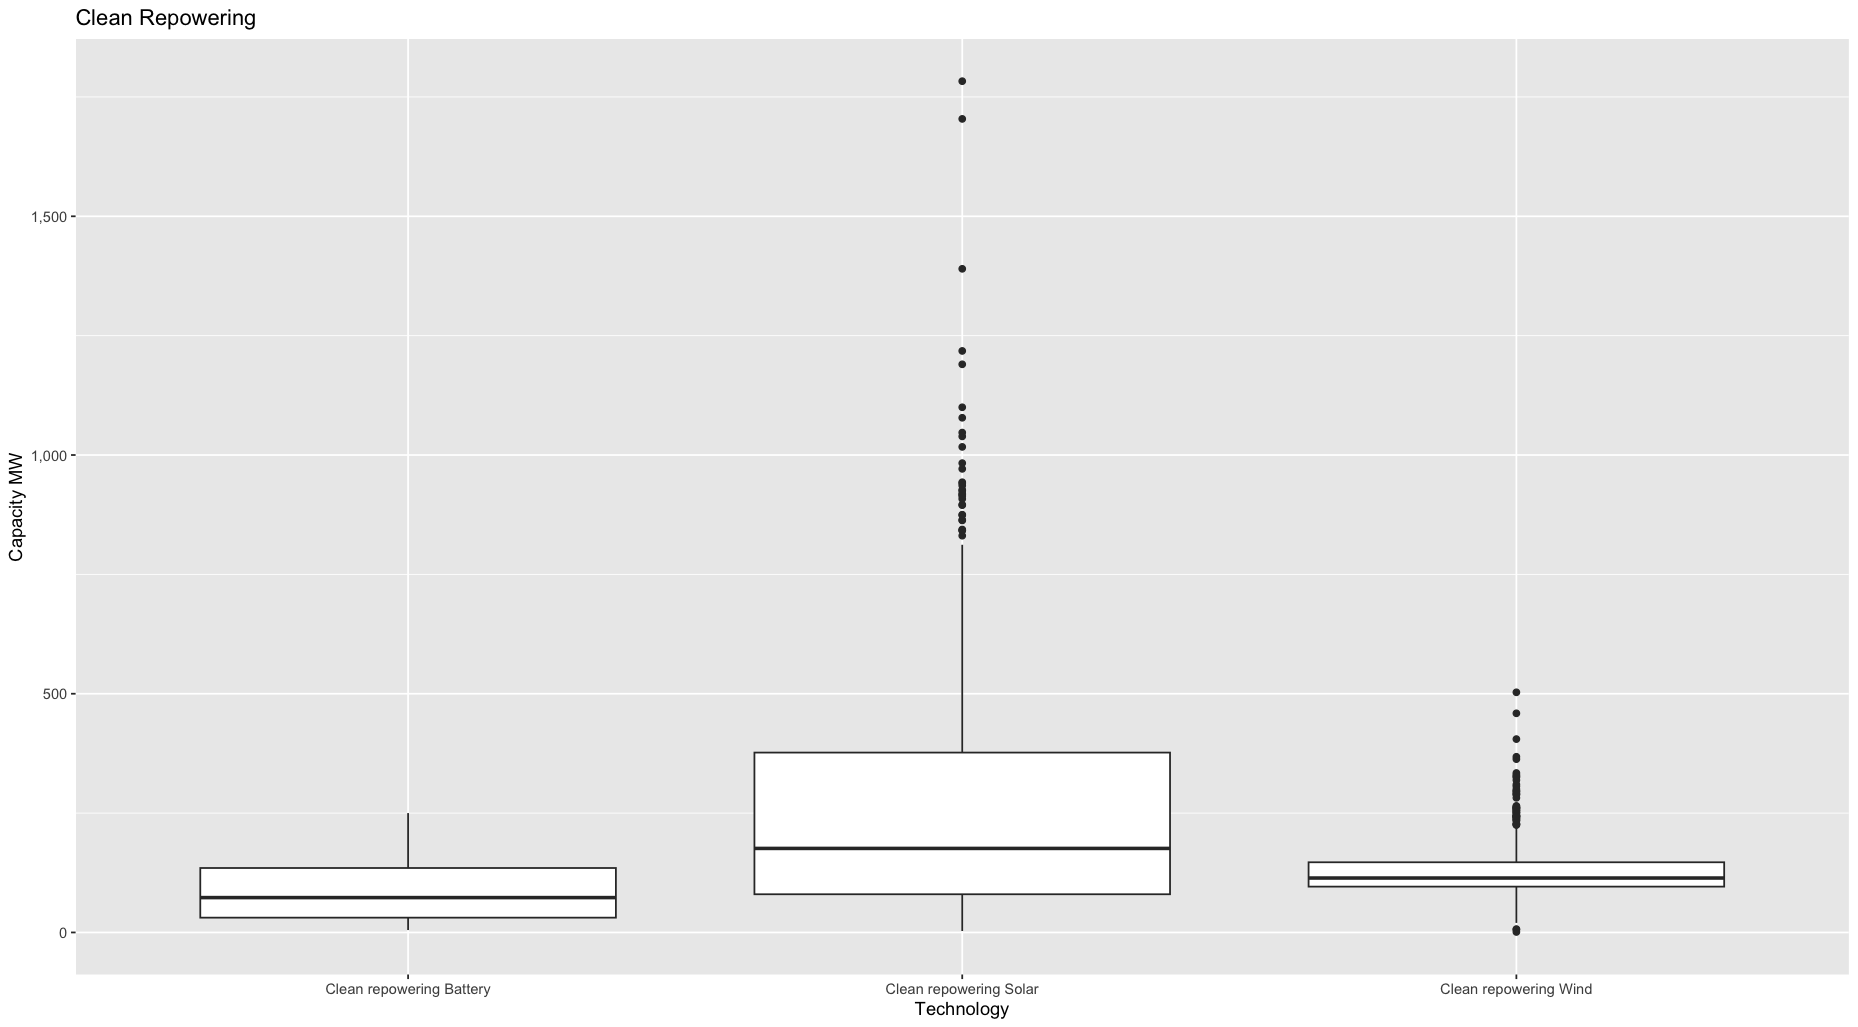
\includegraphics[width=\linewidth]{images/cr_boxplot.png}
  \caption{Clean repowering: Distribution of power}
\end{figure}

\begin{figure}
  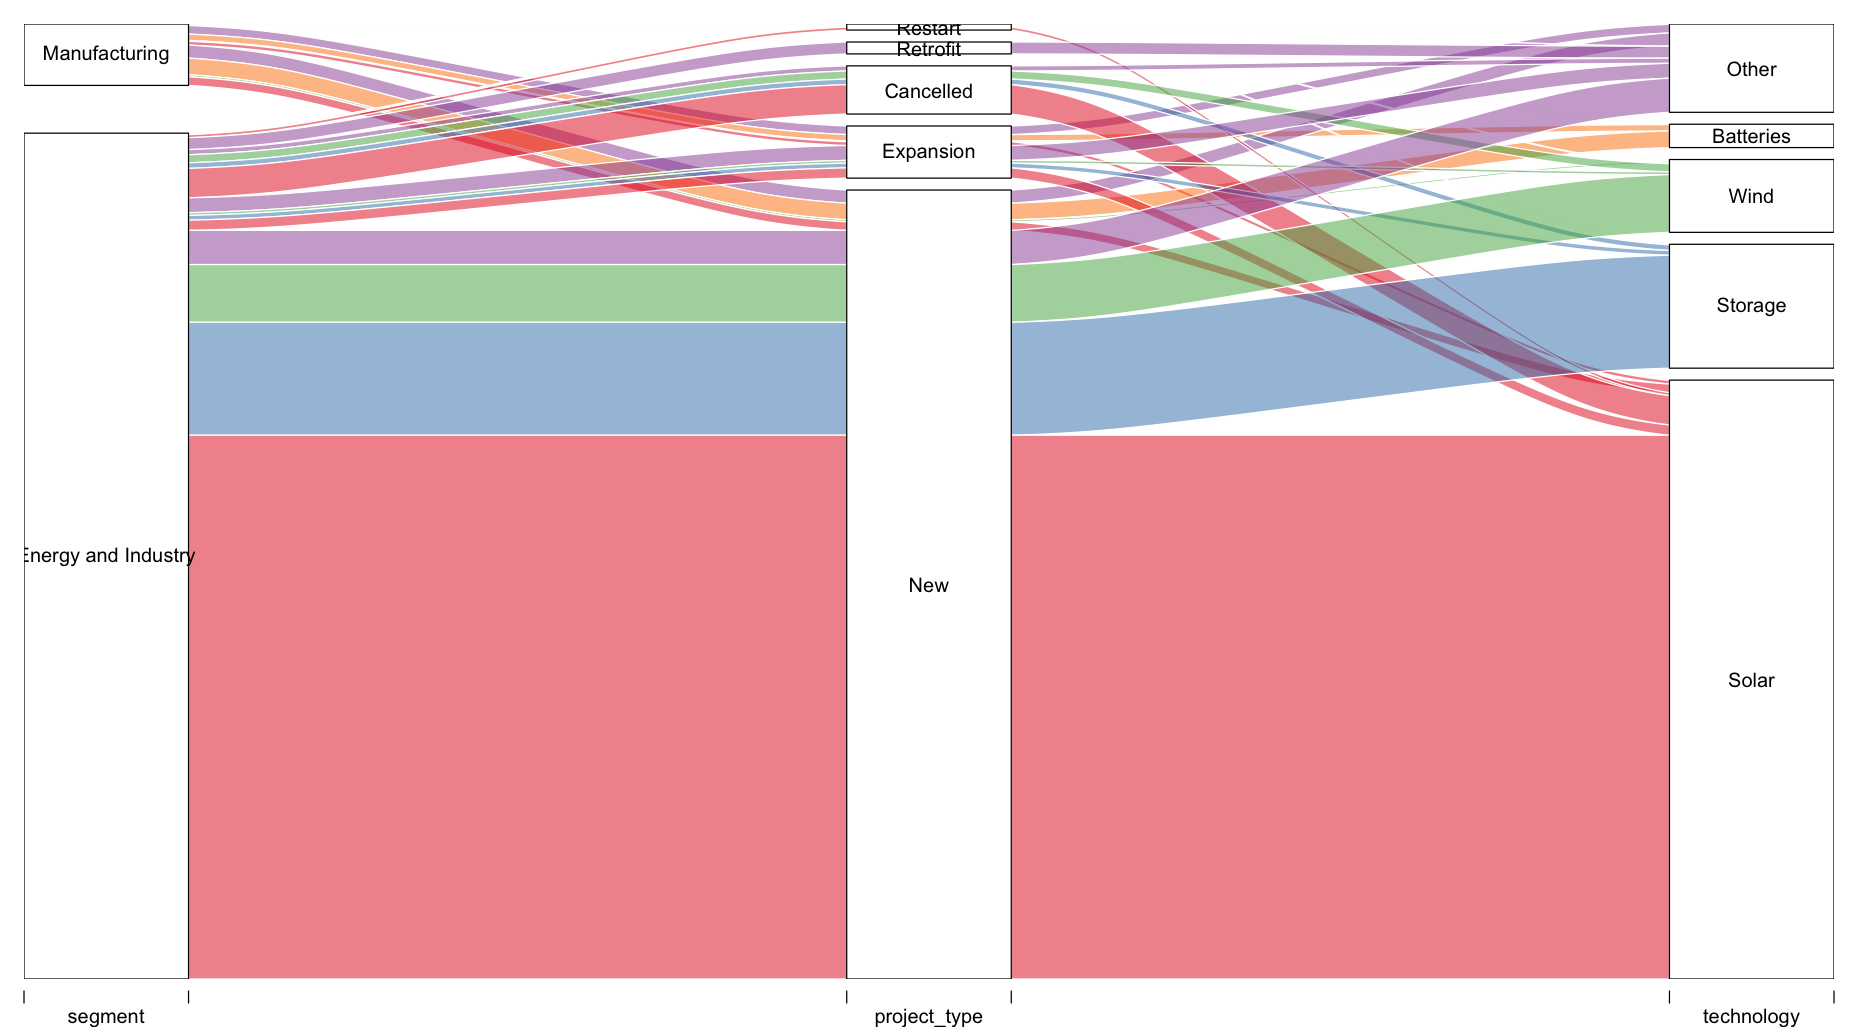
\includegraphics[width=\linewidth]{images/cim_alluvial.png}
  \caption{Clean Investment Monitor: Breakdown of project types}
\end{figure}

The dashboard that we'll create will almost certainly be both interactive, and will feature a map.
(It's worth noting that the reason why Google Looker Studio wasn't doing what I wanted is because I wanted some dots to represent electricity generated, and some to represent CAPEX investments.
Then, I found that GGPlot also doesn't allow multiple metrics to share the same visual metaphor (eg size) while representing entirely different metrics.
So, we'll have to find a flexible tool that allows that kind of thing.)
In this map, I simply z-scored each value-- so, investments are represented in terms of investment standard deviations, and MW is represented in terms of MW standard deviations.

\begin{figure}
  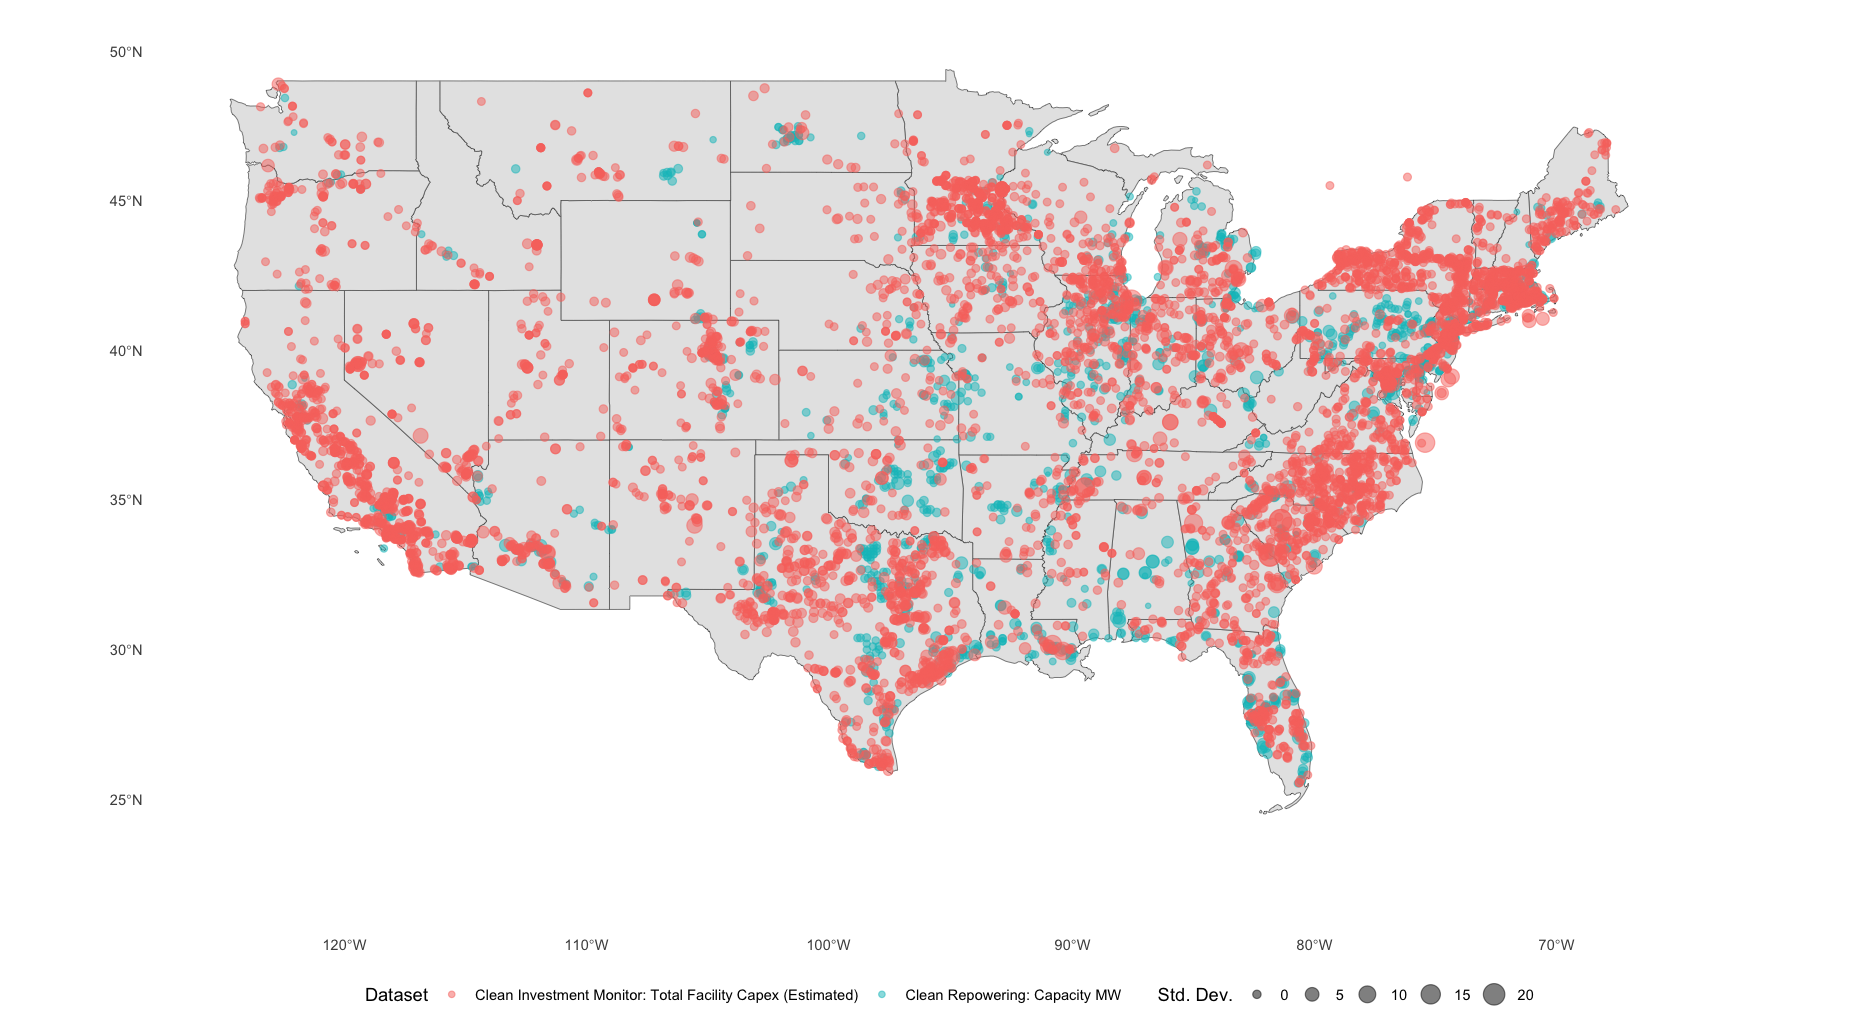
\includegraphics[width=\linewidth]{images/points.png}
  \caption{All of the above points, visualized}
\end{figure}


\section{Useful Metrics}

As we glance at these distributions, our brains will naturally begin to find interesting patterns, and will start to create heuristics. 
This is what I want to explore!
By exploring the questions we four want answered, and the tools that jibe with our minds, we can start to create some pretty cool new tools and metrics.
I believe that it's useful to think in terms of three key metrics, and the relationships between them:
\begin{itemize}
\item MW
\item CAPEX investments
\item Geographic distance
\end{itemize}

The ratio of MW to CAPEX springs to mind, as does the ability to filter clean repowering to a few key kinds of projects, and then sort to the remaining clean investment projects.
But any two opportunities don't really influence each other if they're insufficiently far.

This is why I'm beginning to think not in terms of filtered datasets, but spacially, in terms of a literal triangle tool.
Abstractly, I am thinking of a triangle with three points: MW, CAPEX investments, and Geographic distance (meters, etc). 
I'll keep thinking of how this literal shape can become a functional, useful tool.

\end{document}
